\documentclass{beamer}
\usepackage[utf8]{inputenc}
\usepackage{url}
\usepackage{hyperref}
\graphicspath{{./fig/aula5}}

% Configurando layout para mostrar codigos C++
\usepackage{listings}
\lstset{
  language=HTML,
  basicstyle=\ttfamily\small, 
  keywordstyle=\color{blue}, 
  stringstyle=\color{red}, 
  commentstyle=\color{red}, 
  extendedchars=true, 
  showspaces=false, 
  showstringspaces=false, 
  numbers=left,
  numberstyle=\tiny,
  breaklines=true, 
  backgroundcolor=\color{green!10},
  breakautoindent=true, 
  captionpos=b,
  xleftmargin=0pt,
}
\date{}

\title{Desenvolvimento Web Básico}
\subtitle{Aula 6}

\usetheme{lucid}

\begin{document}
\frame{
 \titlepage
}

%--------------------------------------------------------------------------
\begin{frame}{Na aula de hoje...} 
\tableofcontents 
\end{frame}
%-----------------------------------------
\section{DOM}
\begin{frame}{DOM}
\begin{itemize}
    \item O navegador carrega o HTML e converte o HTML para um DOM (\textit{Document Object Model}). O DOM representa o documento na memória do computador.
    \item O navegador requisita a maioria dos recursos que estão vinculados ao documento HTML, como imagens encorporadas e vídeos, e também, folhas de estilo CSS.
    \item O navegador analisa o CSS encontrado (fetched) e interpreta as diferentes regras por meio dos de seletores, tais como elementos (ex: h1, h2), classes (.myElement), ID (\#myNav), e outros...
    \item Com base nos seletores, o navegador insere as regras de estilização que devem ser aplicadas para cada nó no DOM, e aplica o estilo para os elementos como especificado nas folhas de estilização (este processo intermediário é chamado de render tree ou árvore de renderização).
\end{itemize}
\end{frame}
%---------------------
\begin{frame}{Processamento de página - Esquema}
\begin{center}
		  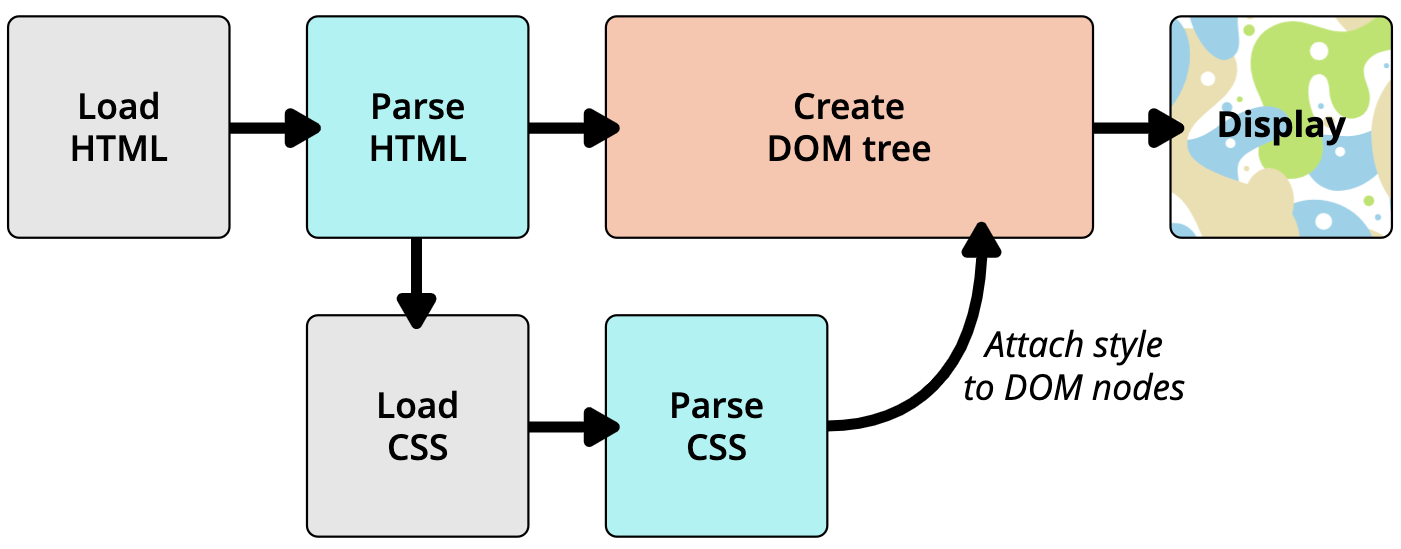
\includegraphics[height=0.45\paperheight]{fig/aula2/dom.png} \\
		   \tiny Fontes: \cite{mdn2023}
	  \end{center}
    
\end{frame}
%-----------------------------------------------------
\begin{frame}{DOM - Exemplo}
\begin{columns}
\begin{column}{0.5\textwidth}
        \begin{center}
		  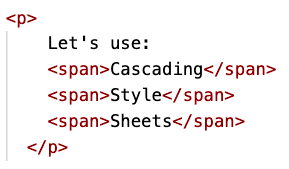
\includegraphics[height=0.4\paperheight]{fig/aula2/dom3.png} \\
		  \tiny{Código HTML}
	  \end{center}
   \end{column}
   \begin{column}{0.5\textwidth}
        \begin{center}
		  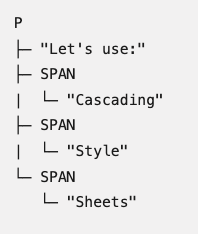
\includegraphics[height=0.4\paperheight]{fig/aula2/dom2.png} \\
		  \tiny{Código CSS}
	  \end{center}
	  
   \end{column}
\end{columns}

\end{frame}
%--------------------------------------------------------------
\section{JavaScript}
\begin{frame}{Por que estudar JavaScript?}
JavaScript é uma das 3 linguagens que todo desenvolvedor WEB deve saber.
	\begin{block}{}
	 \begin{itemize}
	  \item 1. HTML para definir o conteúdo das páginas WEB;
	  \item 2. CSS para definir o layout das páginas WEB;
	  \item 3. JavaScript para programar o comportamento das páginas WEB.
	 \end{itemize}
	\end{block}

\end{frame}
%--------------------------------------------------------------------------
\section{Métodos}
\begin{frame}{getElementById}
	Vejamos um exemplo:\\
	\begin{center}
			
\lstinputlisting[linerange=23-27]{cod/javascript_page.html}
		\end{center}
		\pause O paragrafo com id='demo' recebe o valor da data atual quando o botão recebe um clique.
\end{frame}
%--------------------------------------------------------------------------
\begin{frame}{innerHTML}
A propriedade innerHTML é utilizada para alterar, ou retornar o conteúdo de um elemento HTML.
Vejamos outra forma de utilizar innerHTML.
\begin{center}
			
\lstinputlisting[linerange=30-35]{cod/javascript_page.html}
		\end{center}
		\pause Acrescente este código a nossa página HTML.
\end{frame}
%--------------------------------------------------------------------------
\begin{frame}{innerHTML e function}
Vamos criar uma função que utiliza outra possível aplicação da propriedade innerHTML.
	\begin{center}
		
\lstinputlisting[linerange=36-41]{cod/javascript_page.html}
	\end{center}
	\pause O que essa Função faz?
\end{frame}
%--------------------------------------------------------------------------
\begin{frame}{Alterando a fonte (src) de uma imagem}
Acrescente este código a sua página.
 \begin{center}
	\lstinputlisting[linerange=44-46]{cod/javascript_page.html}
 \end{center}
\end{frame}
%--------------------------------------------------------------------------
\begin{frame}{Alterando a fonte (src) de uma imagem}
Crie um botão:
 \begin{center}
	\lstinputlisting[linerange=47-50]{cod/javascript_page.html}
 \end{center}

\end{frame}
%--------------------------------------------------------------------------
\begin{frame}{Alterando a fonte (src) de uma imagem}
Crie a imagem e, outro botão:
 \begin{center}
	\lstinputlisting[linerange=52-57]{cod/javascript_page.html}
 \end{center}
\pause Ao clicar nos botões o JavaScript edita a fonte da imagem (src) em $<img$
\end{frame}
%--------------------------------------------------------------------------
\begin{frame}{Alterando o estilo de um elemento}
JavaScript também pode editar o estilo de um elemento:
	\begin{center}
			
\lstinputlisting[linerange=59-64]{cod/javascript_page.html}
		\end{center}
\end{frame}
%--------------------------------------------------------------------------
\begin{frame}{Ocultando elementos}
É possível ocultar elementos com JavaScript.
	\begin{center}
		
\lstinputlisting[linerange=65-70]{cod/javascript_page.html}
	\end{center}
\end{frame}
%--------------------------------------------------------------------------
\begin{frame}{Exibindo elementos}
É possível exibir elementos ocultos com JavaScript.
	\begin{center}
		
\lstinputlisting[linerange=72-77]{cod/javascript_page.html}
	\end{center}
\end{frame}
%--------------------------------------------------------------------------
\begin{frame}{Recarregar um HTML}
Utilizando o método document.write() o HTML é totalmente recarregado.
	\begin{center}
		
\lstinputlisting[linerange=81-83]{cod/javascript_page.html}
	\end{center}
\end{frame}

%--------------------------------------------------------------------------
\section{Saídas}
\begin{frame}{Janelas}
Insira o código abaixo na sua página
\begin{center}
	\lstinputlisting[linerange=85-89]{cod/javascript_page.html}
\end{center}
	  
\end{frame}
%--------------------------------------------------------
\begin{frame}{Console}
Insira o código abaixo na sua página
\begin{center}
	\lstinputlisting[linerange=90-93]{cod/javascript_page.html}
\end{center}
Teste. O que mudou?
\pause A propriedade console só é visível ao inspecionar a página, na aba 
console.
\cite{wschool2018js}
	  
\end{frame}
%----------------------------------------------------------------------
\begin{frame}{Variáveis}
 Qual a saída para estes códigos em JavaScript?
 \begin{enumerate}
   \item 5 + 2 + 3;
 	\item "John" + " " + "Doe";
 	\item "5" + 2 + 3;
 \end{enumerate} 	
 \end{frame}

%--------------------------------------------------------------------------
\section{Atividades}
%----------------------------------------------------------
\begin{frame}{Atividade 1}
Divida a página feita em aula em seções e faça uma navbar que permita o usuário navegar na página:

\end{frame}
%-------------------------------------------------------------
\begin{frame}{Atividade 2}
Teste as saídas listadas abaixo e crie um botão para exibir cada uma delas:
	\begin{center}
		  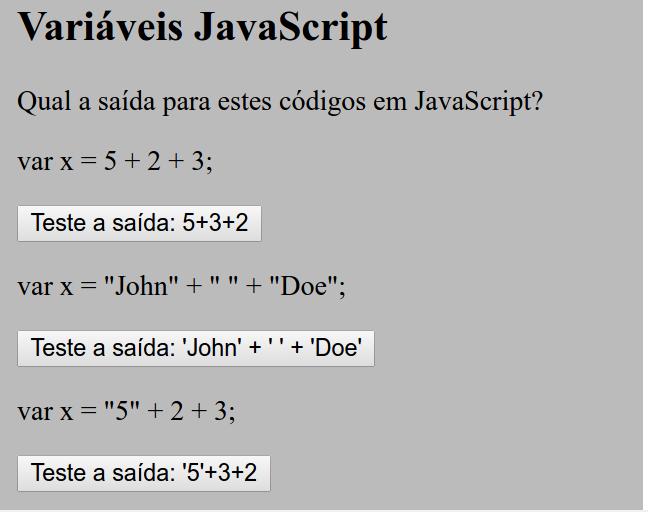
\includegraphics[height=0.6\paperheight]{fig/aula4/teste_js.png} \\
	  \end{center}
\end{frame}
% ---------------------------------------------------------------
\section{Referências}

\begin{frame}{Referências}%[allowframebreaks]
\small
\begin{center}
\tiny
\bibliographystyle{apalike}
\bibliography{ref_aula}
\end{center}
\end{frame}

\end{document}

\end{document}